%begin-include

% Outline of this section
% First we should start with a two-page description of the project with:
% - What are cell signaling pathways
% - What types of computational models we have for these pathways and 
% which one do we use
% - What can we do with those networks and how hard is it to get one to 
% work
% - What are the basic tasks to build a pathway
% - What has Lulu done and what are the limitations of her work
% - How do we intend to surmount those limitations


% Subsection Then we should state the main objectives/challenges of our 
% work
% Subsection Then we should give a short description of the work 


% What are cell signaling pathways and how is it important to study them
% - control how cell behaves in different types of environments
% - cancer cells have bad behavior
% - that's one reason to study signaling networks
Cell signaling pathways are cascades of chemical interactions that 
allow the communication between the cell environment and the 
cell itself. These pathways are also able to regulate many cell 
functions, including DNA replication, cell division and death. We
can observe the functioning of signaling pathways as a mechanism that 
can conform the cell behavior with signals that come from the 
environment conditions in which the cell is placed. The studies of cell 
signaling pathways can lead to determining how cells can respond to 
different stimuli; for instance, with the studies of signaling pathways
activated by a chemical species, one could determine how an unhealthy 
cell would respond to a drug containing this species.

% There are computational models for signaling networks
% - Michaelis Menten equations for chemical interactions
% - With a system of ODES we can then simulate the cell behavior
% - However, the huge number of interactions happening in the cell makes
%   it impossible to consider everything.
% - Therefore we must know 
It is possible to construct mathematical models to represent a set of
chemical reactions and consequently a signaling network. One approach on 
the modeling of those interactions is based on the law of mass action. 
This law proposes that the rate of a chemical reaction is proportional 
to the product of reactants concentrations, i.e. we can calculate the 
concentration change rate of a species in an interaction by calculating 
the product of reactants concentrations, up to a multiplying constant. 
If we consider the set of interactions of a signaling pathway, we can
then come up with a system of ordinary differential equations (ODEs) 
that can model the dynamics of the concentration of each chemical 
species from the pathway. Generally, these systems are complex and 
cumbersome, if not impossible, to be solved analytically, therefore we 
resort on computational tools that apply numerical methods to 
approximate solutions of these systems.

% How do we create these computational models and what should they do?
In this work, we are interested in computational models that can 
reproduce the behavior of signaling networks, comparing simulations
generated by those models to experimental measures, generally based on
Western blot data. The Figure~\ref{fig:signal_pathway_example} shows a
set of interactions as well as parameters of a model of a signaling 
network. To create computational models that are able to simulate the 
behaviour of a signaling pathway, two main tasks need to be 
accomplished.

\begin{figure}[!ht]
\centering 
    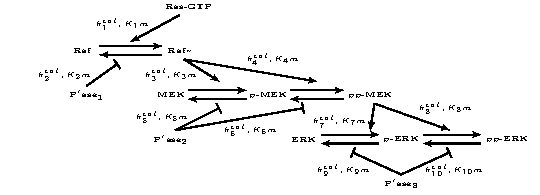
\includegraphics[width=\textwidth]{introduction/csp_example.pdf}
\caption{The above diagram show a hypothesis for a signaling pathway 
    that flows through Raf-MEK-ERK cascade. Names in bold represent 
    chemical species. Names in italic represent parameters of the 
    ordinary differential equation of each interaction.Horizontal arrows
    represent phosphorylation when directed from left to right or 
    dephosphorylation when directed in the opposite direction. Other 
    arrows represent positive feedback if they are directed downwards or 
    negative feedback otherwise. Original image of Marcelo S. Reis et
    al. (2017)~\cite{Reis2017}.}
\label{fig:signal_pathway_example}
\end{figure}

The first task one must complete to create a model is to determine a set 
of interactions that will be considered in the ODE system. Searching for 
pathway maps on the Kyoto Encyclopedia of Genes and Genomes 
(KEGG)~\cite{Kanehisa2000kegg} is a good start for this task. The KEGG 
PATHWAY Database provides manually drawn diagrams that represent 
signaling networks created with experimental evidences. However, it is 
possible that there is no pathway on KEGG that is able to correctly 
represent the biological experiment of interest; for those situations, 
it is necessary to modify the pathway by adding or removing 
interactions. One might reason that we should use as many interactions 
as we can to get a better simulation. Indeed, a model that consider more
reactions is more general and might be able to reproduce different sets
of experimental data. However, being more general may imply in poor or 
computationally infeasible models because of two reasons: first, 
complex models will require more time for a numerical solution 
computation, which may be infeasible due to limited computational 
resources; and second, when considering many interactions, we are also 
considering many parameters (constants of the differential equations 
system), and finding appropriate values for them becomes harder as we 
increase the number of parameters.

The second task is to find values for all the model parameters. We can
highlight two approaches for this task; one can either fetch values for 
these constants from the literature, or one can find values that make 
the model output approximate the experimental observations. For the
first approach, repositories such as BioModels~\cite{le2006biomodels} 
can be used; for the second approach, statistical and optimization
methods are needed. For optimization, it is necessary to define a metric
that can evaluate how close a set of parameters bring the simulation to 
the experimental observation. Only after that it is possible to search 
for the optimal parameter in the parameter space. Statistical inference, 
in the other hand, will usually try to maximize some likelihood function 
(find parameters that makes the data more likely to happen) on a more 
classical approach, while in a Bayesian approach the goal is usually to
compute some posterior distribution for the model parameters (the 
probability of parameter values given the experimental observation).


% However, we might have missed some interactions or even added
% irrelevant ones
After completing both tasks, however, as we mentioned before, we might 
still not have found a pair of model and parameter values that fairly 
approximates the biological experiment of interest. That could indicate 
that the set of chemical interactions chosen for the model is 
incomplete or has interactions that are not relevant for the biological 
experiment. Therefore, it is desirable to construct a systematic method 
of modifying the set of chemical reactions of the model in order to 
find a good set to represent the signaling network.

% Lulu solved it as a combinatorial problem
With the title ``A method to modify molecular signaling networks through
examination of interactome databases"~\cite{Wu15} Lulu Wu presented in 
her masters dissertation a methodology to systematically modify 
computational models of signaling networks to better simulate biological 
experiments. Starting with a model that does not approximate well the 
biological data, this methodology proposes to add to the model
a set of chemical interactions that are relevant for the biochemical 
experiment, and consequently approximate the model simulation to 
experimental data. This set of interactions is a subset of interactions 
from a database created by Wu, joining information from many static 
maps of signaling networks available on KEGG. The choice of this subset 
can be modeled as a combinatorial optimization problem, the feature 
selection problem, in which the search space is the set of all possible 
subsets of interactions (features) to be added. The cost function of 
this problem, however, is not as simple to define as the search space. 
Note that points from the search space do not fully define models, 
because there is still need to define parameter values to produce a 
simulation. Therefore, to analyze the quality of a model, the cost 
function must take into account the set of values for the model 
parameters. As an example, we could define the cost as the minimum 
distance between experimental and model measures considering all 
possibilities of parameter values; however, unfortunately, finding the 
minimizing parameter values is a hard problem.

Since this is a hard problem, the method presented by Wu 
implements a heuristic version of this cost function, moreover, the 
algorithm used to traverse the search space is also a heuristics. The 
cost function heuristics is based on a Simulated Annealing procedure 
that searches for a set of parameter values trying to minimize (as much 
as possible) the distance between model and experimental measures. The 
best found distance times $-1$ is then considered as the cost of the 
model. The size of the search space is the number of all 
possible subsets of interactions to be added, and this number grows
exponentially on the number of interactions from the database. That
explains the need of a heuristic to traverse the search space. This
heuristic is based on the greedy algorithm called Sequential Forward
Selection (SFS)~\cite{Whitney1971}. The heuristic implemented by Wu
selects a fixed number of interactions from the database and then
creates candidate models by adding to the current solution the
respective interaction; then, after evaluating the cost function for
each model, the algorithm moves to the best candidate.

% 1. incompleteness of database (we can use more than KEGG)
% 2. no information about reactions constants
% 3. the algorithm can only add interactions but not remove
% 4. cost function apply penalization randomly and arbitrarily
The results presented on Wu's dissertation show that the method is 
useful when there are only a few differences between the starting model
and a model that closely approximates the biological experiment. This
limitation could be explained by the intrinsic difficulty of the 
problem, which demands fitting complex models with few experimental 
data; however, we would like to highlight three aspects of the work that 
contributes to its limitations. The first aspect is that the constructed 
database could be more nearly complete, adding information from other 
interactome databases, such as STRING~\cite{Szklarczyk2010}, and also by 
adding information about model parameters, i.e. chemical reaction 
constants, that are available in other databases, e.g. the 
SABIO-RK~\cite{Wittig2011} database. Second, the search algorithm used
to modify the models can only add interactions, therefore, if the 
algorithm starts with (or add along the search) a spurious interaction 
on the topology, then the algorithm will not be able to ``regret" that 
interaction even though there might be similar solutions without it with 
better fit. Third, the cost function does not include a proper 
penalization of complex models; the used penalization is based on a 
execution time limit on the simulated annealing procedure, implying on a 
random penalization for more complex models, which typically demand more 
execution time. Without a proper penalization, the algorithm is doomed 
to select overly complex models that, even with a good fit to the 
experimental data, are not likely to reproduce the same experiment
conduced with any kind of perturbation to the biological environment or 
to the data collected.

% To surmount these limitations
% - gather information from many data sources
% - create new search algorithms
% - use Bayesian approach 
We propose on this project to create and test a new method for modifying 
models of signaling networks, based on the work of Wu, and including 
a possible solution to the third aspect mentioned on the last 
paragraph. Although the first and second aspects have potential of 
improvements, we have not prioritized them and, because of the 
complexity of the third aspect, we decided that including the first and 
second aspect would excessively enlarge the scope of this work.
Therefore, we limit our work to a few known cell signaling pathways, and
we only include simple algorithms for traversing the search space. To
the last aspect, which considers the cost function, as our major 
concern in this work, we intend to use Bayesian approaches to rank 
models~\cite{Vyshemirsky2007} based on the likelihood of them to 
reproduce the observed data; if we say $M$ is a model with parameter 
space $\Theta$ and $D$ is a set of observations, then we would like to 
estimate 
\begin{equation*}
    p ({\bm D}|M) = \int_{{\bm \theta} \in \Theta} p ({\bm D} | {\bm
    \theta}, M)p({\bm \theta} | M)d{\bm \theta}, 
\end{equation*}
where $p ({\bm D}|{\bm \theta}, M)$ is the likelihood of data ${\bm D}$,
given that the model $M$ with parameters ${\bm \theta}$ are ``correct'',
which is the same as stating that this model and parameters determine
the behaviour of the cell; $p({\bm \theta} | M)$ is the prior
probability of ${\bm \theta}$; and finally, $p ({\bm D} | M)$ is the
probability of the data being generated by model $M$. This cost function
has as an advantage the fact that models are not ranked using a single
value for parameters, instead, the cost considers all possibilities of
parameters, integrating over the parameter space. Another advantage of
this cost function is that, since it is based on likelihoods of the
model to reproduce data, overly complex models are automatically
penalized.

\section{Objectives}
In this work we propose to implement a methodology that allows us 
to solve the problem of identification of cell signaling pathways as a 
feature selection problem, using a Bayesian approach for the cost
function. This cost function should be able to rank models according to
the likelihood of the experimental data being generated by them. After
the definition and construction of such cost function, we intend to
build small examples of model selection of cell signaling pathways, and
run simple searches on their search spaces, using our chosen cost 
function. Finally, these runs should allow us to get a glance on the
surface that the chosen cost function induces over the search space of
the model selection problem. To achieves these goals, we should
accomplish the following tasks

\begin{enumerate}
    \item{{\bf Study state of the art Bayesian algorithms for signaling
        network model selection}. We have chosen two methodologies to
        study: the first, a work of Liepe et al.~\cite{Liepe2014}, uses
        an Approximate Bayesian Computation approach for ranking models;
        the second, a work of Xu et al.~\cite{Xura20}, uses an
        estimative of the marginal likelihood $p({\bm D}| M)$ to rank
        models.}
    \item{{\bf Implementation and testing of cost functions}. We propose
        to compare both the cost functions used by Liepe and Xu. To test
        the cost function used by Liepe, we should use the software
        ABC-SMC, and to test the cost function used by Xu, we should
        implement our own software, SigNetMS. After the preparation of
        instances, we should test the performance of both software.}
    \item{{\bf Preparation of instances of the identification of cell
        signaling network problem.} After comparing both cost functions,
        we intend to construct instances to test our feature selection
        approach on identification of cell signaling network. These
        instances must be composed by a base model, a small database of
        candidate reactions, and a set of measurements to which our
        candidate models should fit.}
    \item{{\bf Traversal of the search space.} We propose to perform
        walks and runs of simple search algorithms over the search space
        of candidate models for the instances we created. These runs
        will provide us information about the surface that the used cost 
        function induces over the search space. This type of information
        shall be useful for defining new search algorithms for the
        identification of cell signaling pathways.}
\end{enumerate}

\section{Organization}
\begin{itemize}
    \item{\em Chapter 2 (Fundamental Concepts):} we will give more 
        details about the identification of signaling pathway problem. 
        We will show how to obtain experimental data for signaling 
        pathways and how can chain of chemical reactions can be modeled 
        as a system  of differential equations. We close the chapter 
        presenting briefly state of the art methods of model ranking and
        also the  Metropolis-Hastings algorithm, which is a useful tool
        for methods of model ranking.
    \item{\em Chapter 3 (Model Selection Methods):} we will present two
        methodologies that are the state of the art in model selection.
        Both methods are Bayesian approaches, where the first is based
        on Approximate Bayesian Computation, and the second is based on
        the usage of Thermodynamic Integration to create an estimative
        of the marginal likelihood of a model.
    \item{\em Chapter 4 (Development of SigNetMS, a Software for Model
        Ranking):} we present the development of SigNetMS, a software
        that allows model selection by creating an estimative of the
        marginal likelihood of a model. We show the main difficulties
        in implementing this software and how we were able to improve
        its performance.
    \item{\em Chapter 5 (Experiments and Results):} we show two 
        different experiments. The first experiment compares two 
        software for model selection: the first, ABC-SysBio, uses ideas 
        of Approximate Bayesian Computation to rank models; the second,
        SigNetMS, is implemented by us and uses ideas of Thermodynamic
        Integration to create estimates of Marginal Likelihood. After
        comparing both, we create an instance of Model Selection problem
        in terms of a Feature Selection problem, and then we proceed to
        use the chosen software as a score function. With the results of
        such experiment, we are able to get a glance of the surface
        induced by the score function over the search space.
    \item{\em Chapter 6 (Conclusion):} we review all the content
        presented in the previous chapters. We also include a list of 
        contributions related to this work. Finally, we include a list
        of possible suggestions of future work related to this
        dissertation.
\end{itemize}
